%---------- Inleiding ---------------------------------------------------------
\section{Introductie} % The \section*{} command stops section numbering
\label{sec:introductie}
\subsection{Probleemstelling en context}
Om zich te verplaatsen heeft men reeds smartphones met GPS implementaties, wayfinding is hier het toegepaste voorbeeld. Wayfinding is een toepassing om de gewenste locatie en gerichte informatie te vinden met behulp van omgevingsfactoren, het wordt vooral binnen gebruikt. In The Pocket is een bedrijf dat zich focust op digitale producten, zij wensen een applicatie te implementeren dat wayfinding optimaliseert, dit betekent dat er geen fouten meer worden gemaakt bij het wijzen van de weg. 
Om deze toepassing te optimaliseren verlangt men gebruik te maken van AI en AR om omgevingsfactoren te detecteren en te analyseren, bovendien kan men de input vertalen naar de AR omgeving. Als men bijvoorbeeld tegen een muur dreigt te lopen, dan kan AI dit corrigeren.
In deze bachelorproef zal ik een onderzoek voeren dat resulteert in een overzicht van verschillende mogelijke algoritmes en/of aanpakken. Deze zal men kunnen toepassen bij het implementeren van de gewenste applicatie.

\subsection{Motivatie en relevantie onderzoek}
\subsubsection{Motivatie}
De technologieën die worden toegepast in deze probleemstelling bevinden zich in grote mate tot mijn interesse. Een grondig onderzoek zal mijn kennis verrijken en helpen in de toekomst. 
\subsubsection{Relevantie}
Men kan concluderen dat een onderzoek omtrent de samenhang van AI en AR  zeker relevant is. Er wordt veel geëxpermimenteerd met deze techonologieën en een onderzoek kan hierbij een bijdrage leveren.

\subsection{Doelstelling en onderzoeksvraag}
\subsubsection{Doelstelling}
De doelstelling van dit onderzoek is om een duidelijk overzicht te creëren van welke algoritmes en/of aanpakken goede prestaties zullen leveren bij het implementeren in de wayfinding context. Goede prestaties kan men vertalen in een applicatie die zonder fouten, de juiste route zal aangeven.
\subsubsection{Onderzoeksvraag}
De centrale vraag in dit onderzoek is: "Welke bestaande technieken bestaan er reeds om aan de hand van AI en AR de drift in wayfinding te optimaliseren". Hoe kunnen we de wereld rondom de gebruiker herkennen, analyseren en bovendien de input op een bruikbare manier vertalen naar de AR omgeving.

%---------- Stand van zaken ---------------------------------------------------

\section{State-of-the-art}
\label{sec:state-of-the-art}
In het hedendaagse leven wordt er veel gepraat over AI en AR, maar dit gaat niet vaak in samenhang met wayfinding.
Uit de literatuurstudie kan ik concluderen dat er reeds weinig onderzoek is gedaan naar dit bepaald onderwerp, wat dit onderzoek alleen maar interessanter maakt.
Het onderzoek ~\citetitle{Pouria2016} ~\autocite{Pouria2016} is een goede inspiratie, men gebruikt namelijk een gelijkaardige methodiek om het product uit te werken, er zal dan ook meerdere keren naar verwezen worden in mijn onderzoek.
Het onderzoek omtrent ~\citetitle{Zhang2017} ~\autocite{Zhang2017}  omvat een merkwaardige manier om objecten te gaan detecteren, deze manier kan gebruikt worden in een 'indoor navigation task', wat zeer relevant is voor mijn toekomstig onderzoek.
~\citetitle{Liang2015} ~\autocite{Liang2015} is een onderzoek dat een performant objectherkenning algoritme biedt, het resultaat van dit onderzoek zal ik met zekerheid verwerken.
In de paper ~\citetitle{Haikun2017}~\autocite{Haikun2017} bespreekt men een wijze van aanpak dat leidt tot een geoptimaliseerd wayfinding ontwerp met goed geplaatste borden, rekening houdend met de mogelijkheid van het maken van fouten tijdens een navigatie. Aangezien dit reeds een uitgewerkt voorbeeld is van wayfinding zal ik hier rekening mee houden.
Ten slotte is het zeer belangrijk bij wayfinding om de positie steeds tot in puntjes te kunnen waarnemen, \citetitle{Motlagh2009} ~\autocite{Motlagh2009} is een onderzoek dat een oplossing biedt voor dit probleem.
 


% Voor literatuurverwijzingen zijn er twee belangrijke commando's:
% \autocite{KEY} => (Auteur, jaartal) Gebruik dit als de naam van de auteur
%   geen onderdeel is van de zin.
% \textcite{KEY} => Auteur (jaartal)  Gebruik dit als de auteursnaam wel een
%   functie heeft in de zin (bv. ``Uit onderzoek door Doll & Hill (1954) bleek
%   ...'')

%---------- Methodologie ------------------------------------------------------
\section{Methodologie}
\label{sec:methodologie}
Ten eerste zal ik een grondig exploratief onderzoek uitvoeren naar de verschillende mogelijkheden betreffende bestaande methodieken en technieken. Deze zal ik samenstellen in een overzicht waar men de details van elke methodiek/techniek kan raadplegen. Ten tweede zal ik voor één methodiek/techniek een proof-of-concept uitwerken in een praktisch voorbeeld, hieruit kan men het effectieve resultaat bemerken.
Het exploratief onderzoek zal ik oplijsten met R (en markdown), waar men een duidelijk overzicht zal hebben van elke methodiek/techniek met zijn eigenschappen.
Om de proof-of-concept te realiseren zal ik gebruik maken van een IOS-applicatie waar ik AR en AI zal samenbundelen in een praktisch voorbeeld.

%---------- Verwachte resultaten ----------------------------------------------
\section{Verwachte resultaten}
\label{sec:verwachte_resultaten}

Bij het uitvoeren van het exploratief onderzoek reken ik erop een vijftal technieken te vinden die voldoen aan de wensen van de wayfinding context.

De behaalde resultaten zullen worden verzameld door het uitvoeren van experimenten met de betrokken algoritmes en/of aanpakken uit de technieken. Een experiment zal bestaan uit een mogelijke simulatie die het AI -gebeuren zal testen, men zal m.a.w. gaan nakijken of het AI mechanimse effectief een obstakel detecteert.

Ik verwacht dat elke techniek een correctheid heeft van minstens 80 \%, dit beketent dat in 80 \% van de gevallen het algoritme een obstakel zal detecteren. Ik verwacht ook een techniek te vinden die grosso modo 95 \% correct is.

\begin{figure}[H]
	\centering
	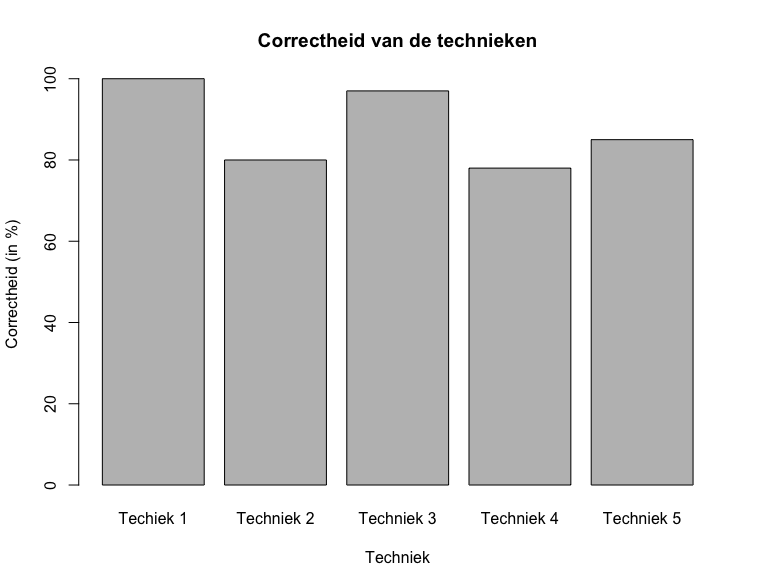
\includegraphics[scale=0.5]{Correctheid_technieken}
	\caption{Verwachte resultaten}
\end{figure}

%---------- Verwachte conclusies ----------------------------------------------
\section{Verwachte conclusies}
\label{sec:verwachte_conclusies}
Door de "jonge leeftijden" van de technoligieën verwacht ik dat het vinden van de nodige documentatie niet van een leien dakje zal lopen, alsook het uitwerken van AI - algoritmes zal zeer complex zijn, maar dit maakt het onderzoek meer uitdagend en zinvol.

Ik hoop een positief resultaat te vinden uit één of meerdere van de experimenten, zodat ik het bedrijf In The Pocket kan helpen bij het vinden van het gepaste algoritme.
